\documentclass[12pt]{article}

% Packages
\usepackage[hidelinks]{hyperref}
\usepackage{geometry}
\usepackage{fancyhdr}
\usepackage{graphicx} 

% Page Geometry
\geometry{a4paper, margin=1in, headheight=14.5pt}

% Header and Footer
\pagestyle{fancy}
\fancyhf{}
\lhead{Discrete Mathematics and Databases}
\rhead{CM12004}
\cfoot{\thepage}

\begin{document}

\title{SQL Databases with Python}
\author{Akim Komarnitskii}
\date{December 15, 2023}
\maketitle
\thispagestyle{fancy}

\begin{figure}[ht]
\section*{Entity–Relationship Model}
\centering
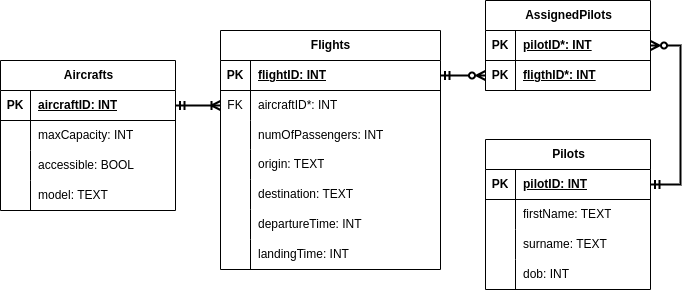
\includegraphics[width=0.8\textwidth]{ERD.png}
\caption{Entity-Relationship Diagram}
\label{fig:erd}
\end{figure}

\section*{Project Link}
Replit link for the project's source code: \url{https://replit.com/@akreg1/cm12004cw2}.

\end{document}
